\documentclass[border=15pt]{standalone}
\usepackage{tikz}
\usepackage{xcolor}
\usepackage{amsmath}
\usetikzlibrary{arrows.meta, calc, decorations.pathreplacing}

%% ── Palette ──────────────────────────────────────────────────────────────────
\definecolor{cWater}{RGB}{31,119,180}
\definecolor{cET}{RGB}{200,50,50}
\definecolor{cHR}{RGB}{44,160,44}
\definecolor{cShade}{RGB}{230,110,0}
\definecolor{cTree}{RGB}{34,120,34}
\definecolor{cSoilTop}{RGB}{193,218,240}
\definecolor{cSoilDeep}{RGB}{108,160,205}
\definecolor{cSoilMono}{RGB}{220,205,185}
\definecolor{cAtm}{RGB}{248,248,250}

\begin{document}
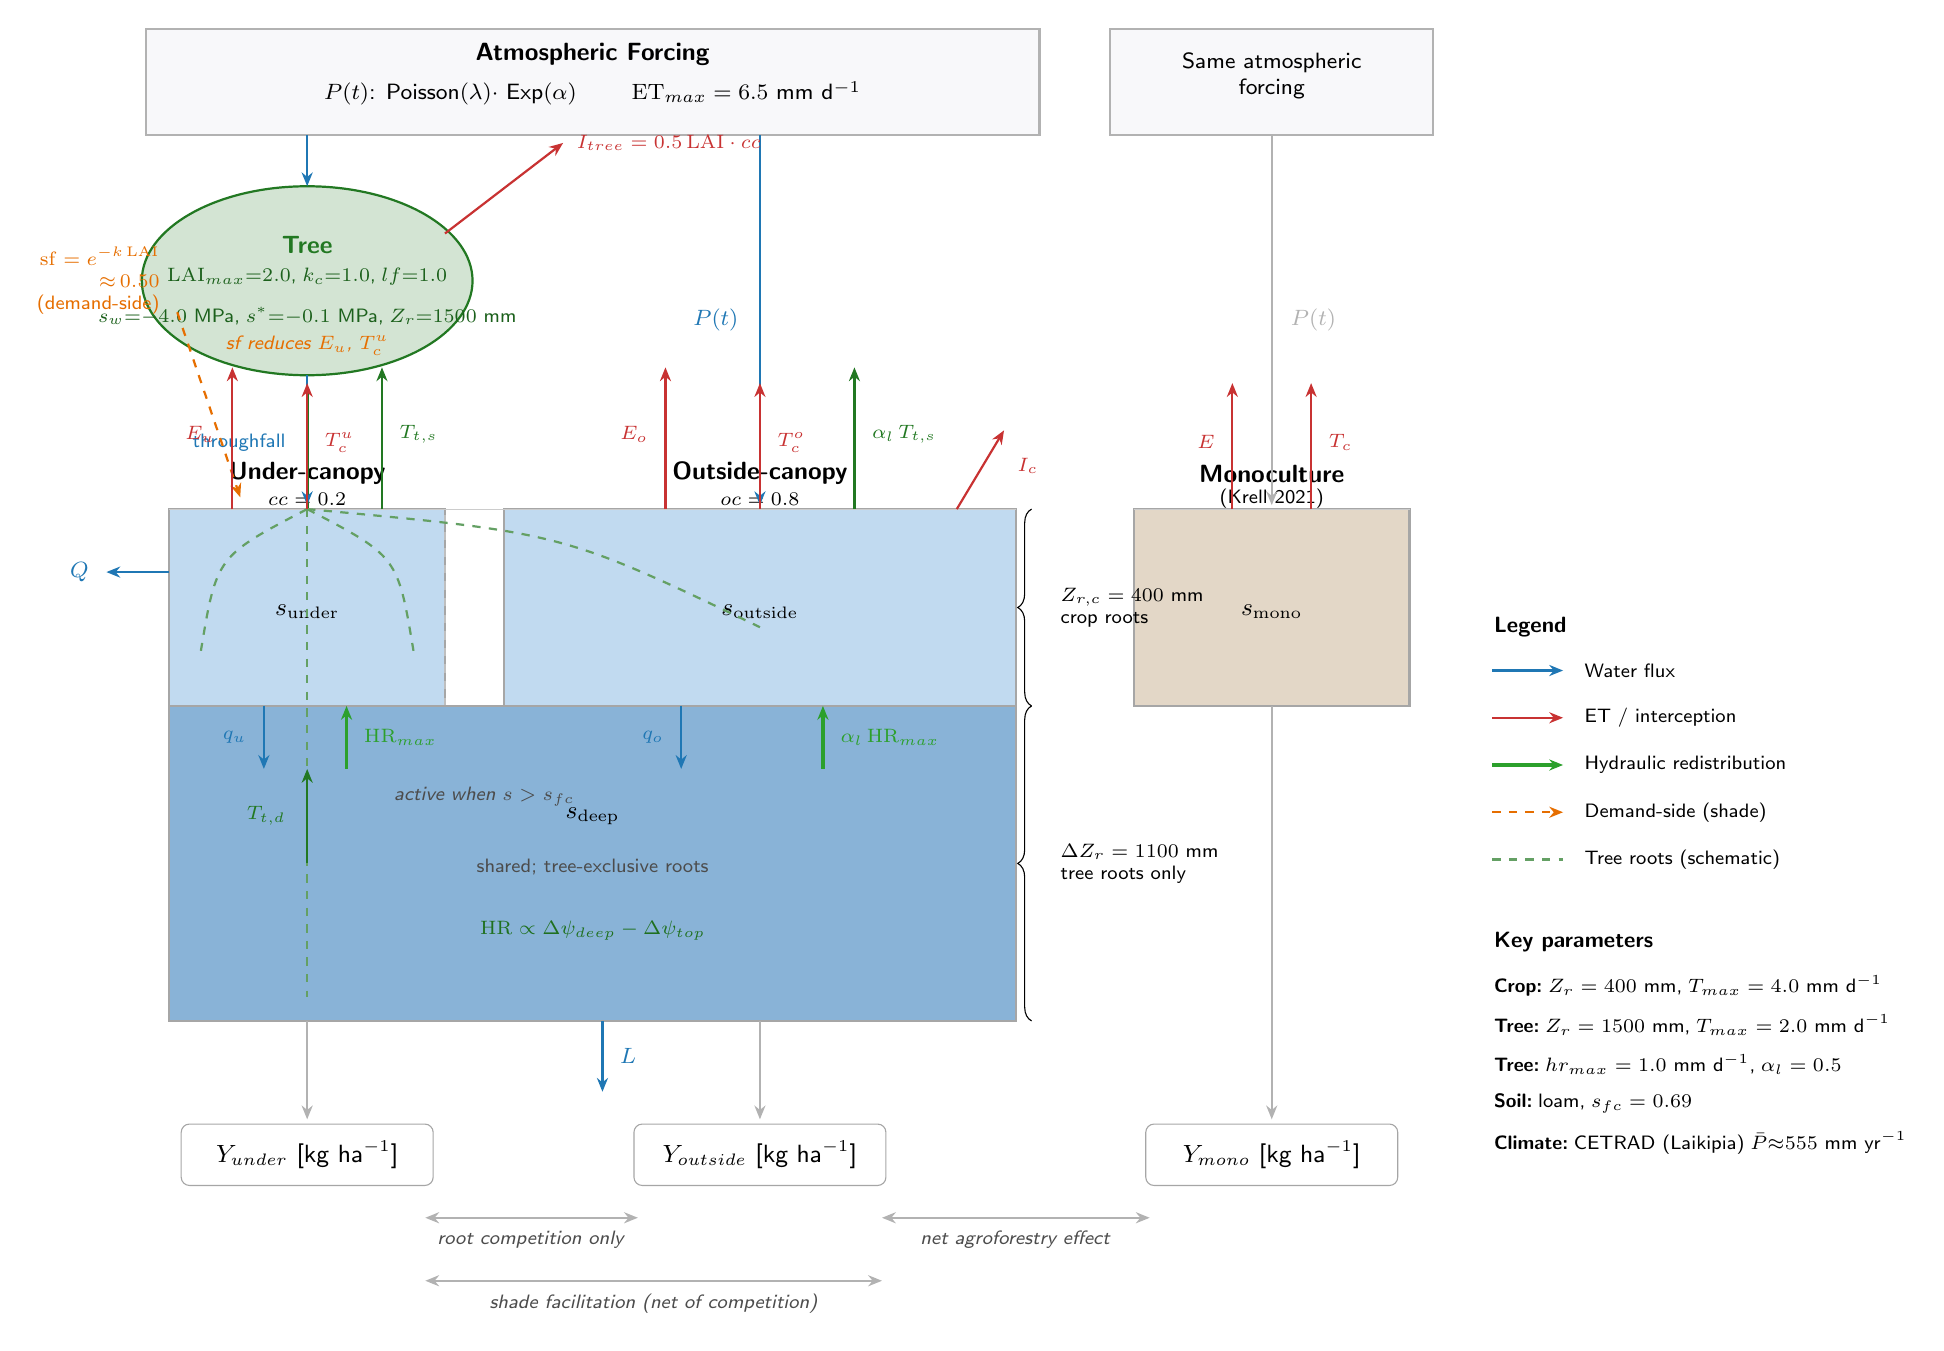
\begin{tikzpicture}[
  >={Stealth[length=5pt,width=4pt]},
  wflow/.style   = {->, thick, cWater},
  eflow/.style   = {->, thick, cET},
  hflow/.style   = {->, very thick, cHR},
  seffect/.style = {->, thick, dashed, cShade},
  roots/.style   = {cTree!70, thick, dashed},
  blabel/.style  = {font=\small\sffamily,  align=center},
  slabel/.style  = {font=\footnotesize\sffamily, align=center},
  tlabel/.style  = {font=\scriptsize\sffamily,   align=center},
]

%% ─────────────────────────────────────────────────────────────────────────────
%% SOIL BOXES
%% ─────────────────────────────────────────────────────────────────────────────

% Under-canopy top layer   [x=0.5..4.0,   y=-2.5..0]
\fill[cSoilTop]  (0.5,-2.5) rectangle (4.0, 0.0);
\draw[gray!70, thick] (0.5,-2.5) rectangle (4.0, 0.0);

% Outside-canopy top layer [x=4.75..11.25, y=-2.5..0]
\fill[cSoilTop]  (4.75,-2.5) rectangle (11.25, 0.0);
\draw[gray!70, thick] (4.75,-2.5) rectangle (11.25, 0.0);

% Zone divider (dashed, under/outside boundary)
\draw[gray!50, dashed, thick] (4.0,-2.5) -- (4.0, 0.0);

% Deep layer (shared)       [x=0.5..11.25, y=-6.5..-2.5]
\fill[cSoilDeep!80] (0.5,-6.5) rectangle (11.25,-2.5);
\draw[gray!70, thick]  (0.5,-6.5) rectangle (11.25,-2.5);

% Monoculture top layer    [x=12.75..16.25, y=-2.5..0]  (no deep layer)
\fill[cSoilMono!80] (12.75,-2.5) rectangle (16.25, 0.0);
\draw[gray!70, thick]   (12.75,-2.5) rectangle (16.25, 0.0);

% Soil surface lines
\draw[gray!40] (0.5,0.0) -- (11.25,0.0);
\draw[gray!40] (12.75,0.0) -- (16.25,0.0);

%% ─────────────────────────────────────────────────────────────────────────────
%% DEPTH BRACES
%% ─────────────────────────────────────────────────────────────────────────────

\draw[decorate, decoration={brace, amplitude=5pt}]
  (11.45,-2.5) -- (11.45, 0.0)
  node[midway, right=7pt, tlabel, align=left]
    {$Z_{r,c} = 400$ mm\\crop roots};

\draw[decorate, decoration={brace, amplitude=5pt}]
  (11.45,-6.5) -- (11.45,-2.5)
  node[midway, right=7pt, tlabel, align=left]
    {$\Delta Z_r = 1100$ mm\\tree roots only};

%% ─────────────────────────────────────────────────────────────────────────────
%% ZONE HEADER LABELS
%% ─────────────────────────────────────────────────────────────────────────────

\node[font=\small\bfseries\sffamily] at (2.25,  0.45) {Under-canopy};
\node[tlabel]                         at (2.25,  0.13) {$cc = 0.2$};

\node[font=\small\bfseries\sffamily] at (8.0,   0.45) {Outside-canopy};
\node[tlabel]                         at (8.0,   0.13) {$oc = 0.8$};

\node[font=\small\bfseries\sffamily] at (14.5,  0.45) {Monoculture};
\node[tlabel]                         at (14.5,  0.13) {(Krell 2021)};

%% ─────────────────────────────────────────────────────────────────────────────
%% STATE VARIABLE LABELS
%% ─────────────────────────────────────────────────────────────────────────────

\node[blabel]                        at (2.25, -1.3)  {$s_{\mathrm{under}}$};
\node[blabel]                        at (8.0,  -1.3)  {$s_{\mathrm{outside}}$};
\node[blabel]                        at (5.875,-3.9)  {$s_{\mathrm{deep}}$};
\node[tlabel, gray!60!black]         at (5.875,-4.55) {shared; tree-exclusive roots};
\node[blabel]                        at (14.5, -1.3)  {$s_{\mathrm{mono}}$};

%% ─────────────────────────────────────────────────────────────────────────────
%% TREE
%% ─────────────────────────────────────────────────────────────────────────────

% Trunk
\draw[cTree, very thick, line cap=round] (2.25, 0.0) -- (2.25, 1.5);

% Canopy ellipse
\fill[cTree!20] (2.25, 2.9) ellipse (2.1 and 1.2);
\draw[cTree, thick] (2.25, 2.9) ellipse (2.1 and 1.2);
\node[font=\small\bfseries\sffamily, cTree] at (2.25, 3.35)
    {Tree};
\node[tlabel, cTree!80!black] at (2.25, 2.95)
    {$\mathrm{LAI}_{max}{=}2.0$,\;$k_c{=}1.0$,\;$lf{=}1.0$};
\node[tlabel, cTree!80!black] at (2.25, 2.45)
    {$s_w{=}{-}4.0$ MPa,\;$s^*{=}{-}0.1$ MPa,\;$Z_r{=}1500$ mm};

% Root lines (schematic)
\draw[roots] (2.25, 0) .. controls (1.1,-0.6) .. (0.9,-1.8);   % under-canopy shallow
\draw[roots] (2.25, 0) .. controls (3.4,-0.6) .. (3.6,-1.8);   % under-canopy shallow
\draw[roots] (2.25, 0) .. controls (5.5,-0.3) .. (8.0,-1.5);   % lateral to outside
\draw[roots] (2.25, 0) -- (2.25,-6.2);                          % deep tap root

%% ─────────────────────────────────────────────────────────────────────────────
%% ATMOSPHERE PANELS
%% ─────────────────────────────────────────────────────────────────────────────

% Agroforestry
\fill[cAtm]        (0.2, 4.75) rectangle (11.55, 6.1);
\draw[gray!60, thick] (0.2, 4.75) rectangle (11.55, 6.1);
\node[font=\small\bfseries\sffamily] at (5.875, 5.78)
    {Atmospheric Forcing};
\node[slabel] at (5.875, 5.28)
    {$P(t)$: Poisson$(\lambda) \cdot$ Exp$(\alpha)$
     \qquad $\mathrm{ET}_{max} = 6.5$ mm d$^{-1}$};

% Monoculture
\fill[cAtm]        (12.45, 4.75) rectangle (16.55, 6.1);
\draw[gray!60, thick] (12.45, 4.75) rectangle (16.55, 6.1);
\node[slabel] at (14.5, 5.5) {Same atmospheric\\forcing};

%% ─────────────────────────────────────────────────────────────────────────────
%% RAINFALL  P(t)
%% ─────────────────────────────────────────────────────────────────────────────

% To tree canopy top (y = 2.9 + 1.2 = 4.1)
\draw[wflow] (2.25, 4.75) -- (2.25, 4.1);

% Outside-canopy: reaches soil directly
\draw[wflow] (8.0, 4.75) -- (8.0, 0.05);
\node[cWater, slabel, left] at (7.85, 2.4) {$P(t)$};

% Monoculture
\draw[wflow, gray!60] (14.5, 4.75) -- (14.5, 0.05);
\node[gray!60, slabel, right] at (14.62, 2.4) {$P(t)$};

%% ─────────────────────────────────────────────────────────────────────────────
%% TREE INTERCEPTION  &  THROUGHFALL
%% ─────────────────────────────────────────────────────────────────────────────

% Interception exits canopy (diagonal up-right)
\draw[eflow] (4.0, 3.5) -- (5.5, 4.65);
\node[cET, tlabel, right] at (5.55, 4.65)
    {$I_{tree} = 0.5\,\mathrm{LAI}\cdot cc$};

% Throughfall (canopy bottom y=1.7 → soil surface)
\draw[wflow] (2.25, 1.7) -- (2.25, 0.05);
\node[cWater, tlabel, left] at (2.1, 0.85) {throughfall};

%% ─────────────────────────────────────────────────────────────────────────────
%% SHADE EFFECT  (demand-side; dashed orange)
%% ─────────────────────────────────────────────────────────────────────────────

\draw[seffect] (0.6, 2.5) -- (1.4, 0.15);
\node[cShade, tlabel, left, align=right] at (0.5, 2.9)
    {$\mathrm{sf} = e^{-k\,\mathrm{LAI}}$\\${\approx}\,0.50$\\(demand-side)};

%% ─────────────────────────────────────────────────────────────────────────────
%% ET LOSSES FROM TOP LAYERS
%% ─────────────────────────────────────────────────────────────────────────────

% Under-canopy: E_u (shade-reduced), T_crop^u (shade-reduced), T_tree_shallow
\draw[eflow]        (1.3,  0.0) -- (1.3,  1.8);
\node[cET,   tlabel, left]  at (1.2,  0.95) {$E_u$};
\draw[eflow]        (2.25, 0.0) -- (2.25, 1.6);
\node[cET,   tlabel, right] at (2.35, 0.85) {$T_c^u$};
\draw[eflow, cTree] (3.2,  0.0) -- (3.2,  1.8);
\node[cTree, tlabel, right] at (3.3,  0.95) {$T_{t,s}$};
\node[cShade, tlabel] at (2.25, 2.08)
    {\textit{sf reduces $E_u$, $T_c^u$}};

% Outside-canopy: E_o (full), T_crop^o (full), alpha_lat * T_tree_shallow
\draw[eflow]        (6.8, 0.0) -- (6.8, 1.8);
\node[cET,   tlabel, left]  at (6.7, 0.95) {$E_o$};
\draw[eflow]        (8.0, 0.0) -- (8.0, 1.6);
\node[cET,   tlabel, right] at (8.1, 0.85) {$T_c^o$};
\draw[eflow, cTree] (9.2, 0.0) -- (9.2, 1.8);
\node[cTree, tlabel, right] at (9.3, 0.95) {$\alpha_l\,T_{t,s}$};

% Outside-canopy crop interception (brief)
\draw[eflow] (10.5, 0.0) -- (11.1, 1.0);
\node[cET, tlabel, right] at (11.15, 0.55) {$I_c$};

% Monoculture: E, T_crop
\draw[eflow] (14.0, 0.0) -- (14.0, 1.6);
\node[cET, tlabel, left]  at (13.9, 0.85) {$E$};
\draw[eflow] (15.0, 0.0) -- (15.0, 1.6);
\node[cET, tlabel, right] at (15.1, 0.85) {$T_c$};

%% ─────────────────────────────────────────────────────────────────────────────
%% RUNOFF
%% ─────────────────────────────────────────────────────────────────────────────

\draw[wflow] (0.5, -0.8) -- (-0.3, -0.8);
\node[cWater, slabel, left] at (-0.4, -0.8) {$Q$};

%% ─────────────────────────────────────────────────────────────────────────────
%% PERCOLATION  (top layer → deep layer)
%% ─────────────────────────────────────────────────────────────────────────────

\draw[wflow] (1.7, -2.5) -- (1.7, -3.3);
\node[cWater, tlabel, left]  at (1.6, -2.9) {$q_u$};

\draw[wflow] (7.0, -2.5) -- (7.0, -3.3);
\node[cWater, tlabel, left]  at (6.9, -2.9) {$q_o$};

\node[tlabel, gray!60!black] at (4.5, -3.65)
    {\textit{active when $s > s_{fc}$}};

%% ─────────────────────────────────────────────────────────────────────────────
%% HYDRAULIC REDISTRIBUTION  HR  (deep → top)
%% ─────────────────────────────────────────────────────────────────────────────

% Full HR to under-canopy
\draw[hflow] (2.75, -3.3) -- (2.75, -2.5);
\node[cHR, tlabel, right] at (2.85, -2.9) {$\mathrm{HR}_{max}$};

% Scaled HR to outside-canopy
\draw[hflow] (8.8, -3.3) -- (8.8, -2.5);
\node[cHR, tlabel, right] at (8.9, -2.9) {$\alpha_l\,\mathrm{HR}_{max}$};

% Driving force annotation
\node[cHR!70!black, tlabel] at (5.875, -5.35)
    {$\mathrm{HR} \propto \Delta\psi_{deep} - \Delta\psi_{top}$};

%% ─────────────────────────────────────────────────────────────────────────────
%% TREE DEEP TRANSPIRATION  (from deep layer)
%% ─────────────────────────────────────────────────────────────────────────────

\draw[eflow, cTree] (2.25, -4.5) -- (2.25, -3.3);
\node[cTree, tlabel, left] at (2.1, -3.9) {$T_{t,d}$};

%% ─────────────────────────────────────────────────────────────────────────────
%% DEEP DRAINAGE / LEAKAGE  L
%% ─────────────────────────────────────────────────────────────────────────────

\draw[wflow] (6.0, -6.5) -- (6.0, -7.4);
\node[cWater, slabel, right] at (6.1, -6.95) {$L$};

%% ─────────────────────────────────────────────────────────────────────────────
%% YIELD OUTPUT
%% ─────────────────────────────────────────────────────────────────────────────

\draw[->, thick, gray!60] (2.25, -6.5)  -- (2.25, -7.75);
\draw[->, thick, gray!60] (8.0,  -6.5)  -- (8.0,  -7.75);
\draw[->, thick, gray!60] (14.5, -2.5)  -- (14.5, -7.75);

\node[draw=gray!70, rounded corners=3pt, fill=white,
      minimum width=3.2cm, minimum height=0.78cm, blabel]
    at (2.25,  -8.2) {$Y_{under}$ [kg ha$^{-1}$]};

\node[draw=gray!70, rounded corners=3pt, fill=white,
      minimum width=3.2cm, minimum height=0.78cm, blabel]
    at (8.0,   -8.2) {$Y_{outside}$ [kg ha$^{-1}$]};

\node[draw=gray!70, rounded corners=3pt, fill=white,
      minimum width=3.2cm, minimum height=0.78cm, blabel]
    at (14.5,  -8.2) {$Y_{mono}$ [kg ha$^{-1}$]};

%% Decomposition double-arrows
\draw[<->, thick, gray!60] (3.75, -9.0) -- (6.45, -9.0);
\node[tlabel, gray!60!black, below] at (5.1, -9.05)
    {\textit{root competition only}};

\draw[<->, thick, gray!60] (9.55, -9.0) -- (12.95, -9.0);
\node[tlabel, gray!60!black, below] at (11.25, -9.05)
    {\textit{net agroforestry effect}};

\draw[<->, thick, gray!60] (3.75, -9.8) -- (9.55, -9.8);
\node[tlabel, gray!60!black, below] at (6.65, -9.85)
    {\textit{shade facilitation (net of competition)}};

%% ─────────────────────────────────────────────────────────────────────────────
%% LEGEND  (right side, clear of all elements)
%% ─────────────────────────────────────────────────────────────────────────────

\begin{scope}[shift={(17.2, -1.5)}]
  \node[font=\footnotesize\bfseries\sffamily, anchor=west] at (0, 0)
      {Legend};
  \draw[wflow]    (0.1, -0.55) -- (1.0, -0.55);
  \node[tlabel, anchor=west] at (1.15, -0.55) {Water flux};
  \draw[eflow]    (0.1, -1.15) -- (1.0, -1.15);
  \node[tlabel, anchor=west] at (1.15, -1.15) {ET / interception};
  \draw[hflow]    (0.1, -1.75) -- (1.0, -1.75);
  \node[tlabel, anchor=west] at (1.15, -1.75) {Hydraulic redistribution};
  \draw[seffect]  (0.1, -2.35) -- (1.0, -2.35);
  \node[tlabel, anchor=west] at (1.15, -2.35) {Demand-side (shade)};
  \draw[roots]    (0.1, -2.95) -- (1.0, -2.95);
  \node[tlabel, anchor=west] at (1.15, -2.95) {Tree roots (schematic)};
\end{scope}

%% ─────────────────────────────────────────────────────────────────────────────
%% PARAMETER INSET  (right side, below legend)
%% ─────────────────────────────────────────────────────────────────────────────

\begin{scope}[shift={(17.2, -5.5)}]
  \node[font=\footnotesize\bfseries\sffamily, anchor=west] at (0, 0)
      {Key parameters};
  \node[tlabel, anchor=west] at (0, -0.55)
      {\textbf{Crop:}\;$Z_r=400$ mm,\;$T_{max}=4.0$ mm d$^{-1}$};
  \node[tlabel, anchor=west] at (0, -1.05)
      {\textbf{Tree:}\;$Z_r=1500$ mm,\;$T_{max}=2.0$ mm d$^{-1}$};
  \node[tlabel, anchor=west] at (0, -1.55)
      {\textbf{Tree:}\;$hr_{max}=1.0$ mm d$^{-1}$,\;$\alpha_l=0.5$};
  \node[tlabel, anchor=west] at (0, -2.05)
      {\textbf{Soil:}\;loam,\;$s_{fc}=0.69$};
  \node[tlabel, anchor=west] at (0, -2.55)
      {\textbf{Climate:}\;CETRAD (Laikipia)\;$\bar{P}{\approx}555$ mm yr$^{-1}$};
\end{scope}

\end{tikzpicture}
\end{document}
